% Options for packages loaded elsewhere
\PassOptionsToPackage{unicode}{hyperref}
\PassOptionsToPackage{hyphens}{url}
\documentclass[
]{article}
\usepackage{xcolor}
\usepackage[margin=2cm]{geometry}
\usepackage{amsmath,amssymb}
\setcounter{secnumdepth}{-\maxdimen} % remove section numbering
\usepackage{iftex}
\ifPDFTeX
  \usepackage[T1]{fontenc}
  \usepackage[utf8]{inputenc}
  \usepackage{textcomp} % provide euro and other symbols
\else % if luatex or xetex
  \usepackage{unicode-math} % this also loads fontspec
  \defaultfontfeatures{Scale=MatchLowercase}
  \defaultfontfeatures[\rmfamily]{Ligatures=TeX,Scale=1}
\fi
\usepackage{lmodern}
\ifPDFTeX\else
  % xetex/luatex font selection
\fi
% Use upquote if available, for straight quotes in verbatim environments
\IfFileExists{upquote.sty}{\usepackage{upquote}}{}
\IfFileExists{microtype.sty}{% use microtype if available
  \usepackage[]{microtype}
  \UseMicrotypeSet[protrusion]{basicmath} % disable protrusion for tt fonts
}{}
\makeatletter
\@ifundefined{KOMAClassName}{% if non-KOMA class
  \IfFileExists{parskip.sty}{%
    \usepackage{parskip}
  }{% else
    \setlength{\parindent}{0pt}
    \setlength{\parskip}{6pt plus 2pt minus 1pt}}
}{% if KOMA class
  \KOMAoptions{parskip=half}}
\makeatother
\usepackage{longtable,booktabs,array}
\usepackage{calc} % for calculating minipage widths
% Correct order of tables after \paragraph or \subparagraph
\usepackage{etoolbox}
\makeatletter
\patchcmd\longtable{\par}{\if@noskipsec\mbox{}\fi\par}{}{}
\makeatother
% Allow footnotes in longtable head/foot
\IfFileExists{footnotehyper.sty}{\usepackage{footnotehyper}}{\usepackage{footnote}}
\makesavenoteenv{longtable}
\usepackage{graphicx}
\makeatletter
\newsavebox\pandoc@box
\newcommand*\pandocbounded[1]{% scales image to fit in text height/width
  \sbox\pandoc@box{#1}%
  \Gscale@div\@tempa{\textheight}{\dimexpr\ht\pandoc@box+\dp\pandoc@box\relax}%
  \Gscale@div\@tempb{\linewidth}{\wd\pandoc@box}%
  \ifdim\@tempb\p@<\@tempa\p@\let\@tempa\@tempb\fi% select the smaller of both
  \ifdim\@tempa\p@<\p@\scalebox{\@tempa}{\usebox\pandoc@box}%
  \else\usebox{\pandoc@box}%
  \fi%
}
% Set default figure placement to htbp
\def\fps@figure{htbp}
\makeatother
\ifLuaTeX
  \usepackage{luacolor}
  \usepackage[soul]{lua-ul}
\else
  \usepackage{soul}
\fi
\setlength{\emergencystretch}{3em} % prevent overfull lines
\providecommand{\tightlist}{%
  \setlength{\itemsep}{0pt}\setlength{\parskip}{0pt}}
\usepackage{bookmark}
\IfFileExists{xurl.sty}{\usepackage{xurl}}{} % add URL line breaks if available
\urlstyle{same}
\hypersetup{
  pdftitle={Technology of Microelectronic- Important values},
  pdfauthor={Thomas Debelle},
  hidelinks,
  pdfcreator={LaTeX via pandoc}}

\title{Technology of Microelectronic- Important values}
\author{Thomas Debelle}
\date{}

\begin{document}
\maketitle

\begin{itemize}
\tightlist
\item
  \hyperref[first-chapter]{First Chapter}

  \begin{itemize}
  \tightlist
  \item
    \hyperref[silicon-properties]{Silicon properties}
  \item
    \hyperref[boule-making]{Boule making}
  \end{itemize}
\item
  \hyperref[2-lithography]{2 Lithography}

  \begin{itemize}
  \tightlist
  \item
    \hyperref[resist-spinning]{Resist spinning}
  \item
    \hyperref[optic]{Optic}
  \item
    \hyperref[mask-and-formulas]{Mask and formulas}
  \item
    \hyperref[lights]{Lights}
  \item
    \hyperref[double-patterning]{Double patterning}
  \item
    \hyperref[euv]{EUV}
  \end{itemize}
\item
  \hyperref[4-oxidation-wet-dry]{4 Oxidation, wet, dry}

  \begin{itemize}
  \tightlist
  \item
    \hyperref[thermal-oxidation]{Thermal oxidation}
  \item
    \hyperref[locos]{LOCOS}
  \item
    \hyperref[sti]{STI}
  \item
    \hyperref[doping]{Doping}
  \item
    \hyperref[ion-implantation]{Ion Implantation}
  \end{itemize}
\item
  \hyperref[5-etching-wet-dry-plasma-drie]{5 Etching, wet, dry, plasma,
  DRIE}

  \begin{itemize}
  \tightlist
  \item
    \hyperref[anisotropic]{Anisotropic}
  \end{itemize}
\item
  \hyperref[6-interconnect]{6 Interconnect}

  \begin{itemize}
  \tightlist
  \item
    \hyperref[electromigration]{Electromigration}
  \item
    \hyperref[interconnect]{Interconnect}
  \end{itemize}
\item
  \hyperref[7-ic-processing-overview]{7 Ic Processing Overview}

  \begin{itemize}
  \tightlist
  \item
    \hyperref[al-vs-poly]{Al vs poly}
  \item
    \hyperref[latch-up-issue]{Latch-up issue}
  \item
    \hyperref[hot-carrier-effect]{Hot carrier effect}
  \item
    \hyperref[contacting-issues]{Contacting issues}
  \end{itemize}
\item
  \hyperref[8-packaging]{8 Packaging}
\end{itemize}

\subsection{First Chapter}\label{first-chapter}

Positive etch mask = exposed area will be removed. Negative vice versa.

\begin{longtable}[]{@{}cc@{}}
\toprule\noalign{}
Wafer Size & Thickness \\
\midrule\noalign{}
\endhead
\bottomrule\noalign{}
\endlastfoot
4'' & 400 \(\mu m\) \\
8-12'' & 1.2 mm \\
\end{longtable}

\subsubsection{Silicon properties}\label{silicon-properties}

Cheap and strong, fragile. Resistivity 0.001 - 20 \(k\Omega /cm\). Can
be SCS, poly or amorphous. Can deform without cracking for quite some
time.

\pandocbounded{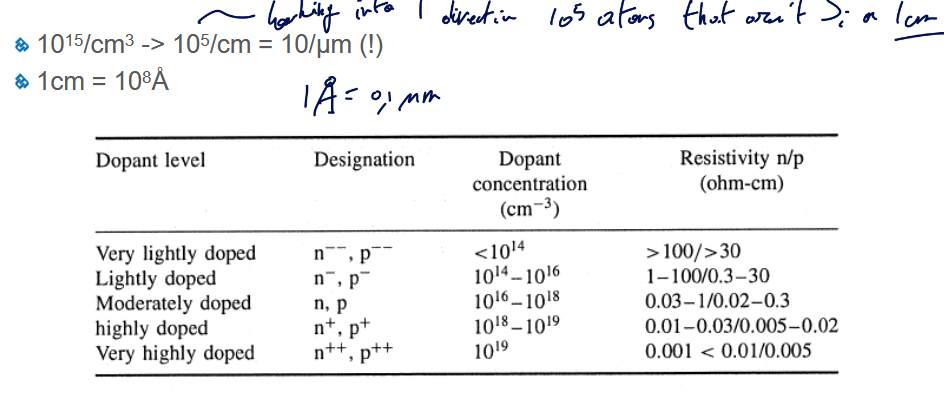
\includegraphics[keepaspectratio]{image.png}}\{.width=50\%\}

In a Si cube we have 8 atoms inside the cell. with:

\[
Volume = (.543nm)^3 \qquad \frac{8}{Volume} = 5\cdot 10^{22} atoms/cm^3
\]

SCS has a purity up to 11 nines ! and is 2 FCC lattices displaced by
.25, .25, .25.

\subsubsection{Boule making}\label{boule-making}

To create a Boule we can use a Czochralski pulling at 1420C. The pull
rate is around \textbf{mm/min}. 30 hours for 2m + 30 hours for cooling!

\paragraph{Wafer treatment}\label{wafer-treatment}

First we have to cut then to get a perfect wafer we will have:

\begin{enumerate}
\def\labelenumi{\arabic{enumi}.}
\tightlist
\item
  Lapping: \(20 \mu m\)/side
\item
  Edge profiling: makes edge cleaner
\item
  Etching (chemical): \(20 \mu m\)/side
\item
  Polishing (CMP): \(25 \mu m\)/side
\end{enumerate}

\pandocbounded{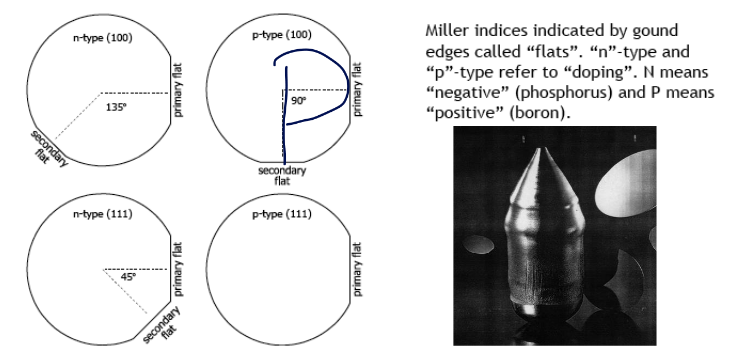
\includegraphics[keepaspectratio]{image-1.png}}\{.width=50\%\}

A boat can contain between 12 to 24 wafer.

\pandocbounded{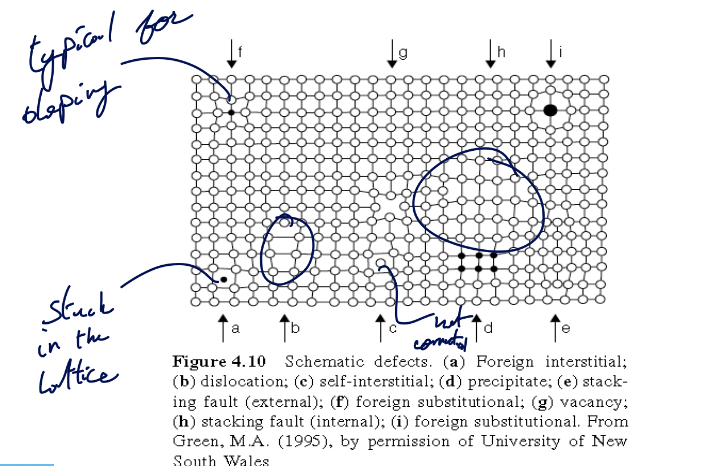
\includegraphics[keepaspectratio]{image-2.png}}\{.width=50\%\}

We drop some die on the chips that aren't good due to a defect. Lower
defect ratio allows to put bigger transistor. But going smaller isn't
always the best as the interconnect cost can quickly ramp up as we go
too small. So optimization process between Packaging and reliability
(yield).

\pandocbounded{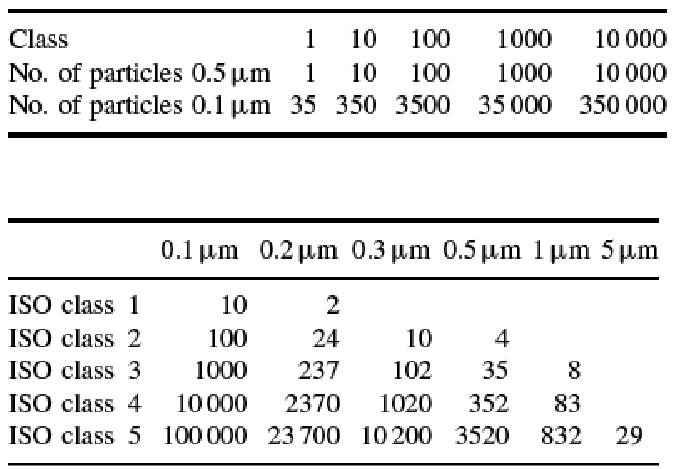
\includegraphics[keepaspectratio]{image-3.png}}\{.width=50\%\}

\pandocbounded{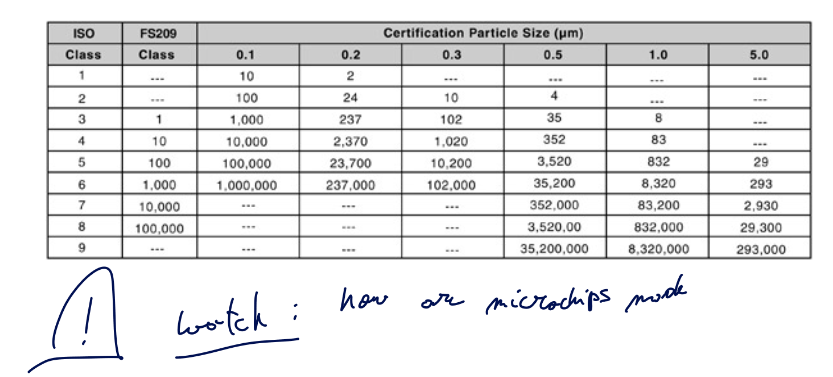
\includegraphics[keepaspectratio]{image-4.png}}\{.width=50\%\}

Class ISO:

\begin{itemize}
\tightlist
\item
  10.000: PCB, packaging
\item
  1.000: MEMS, packaging, HDD
\item
  100: MEMS, RF/Photonic ICs
\item
  10: IC
\end{itemize}

\subsection{2 Lithography}\label{lithography}

\pandocbounded{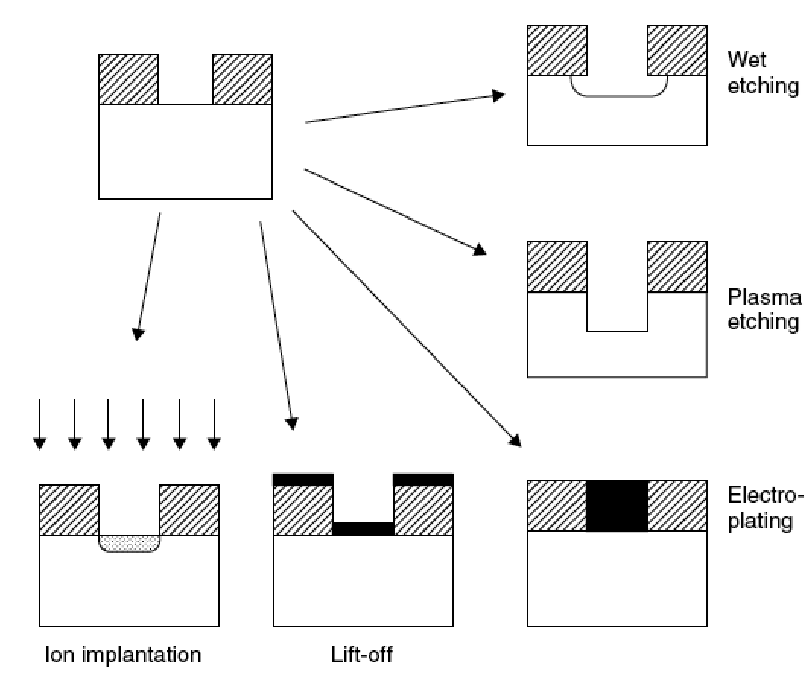
\includegraphics[keepaspectratio]{image-5.png}}\{.width=50\%\}

\pandocbounded{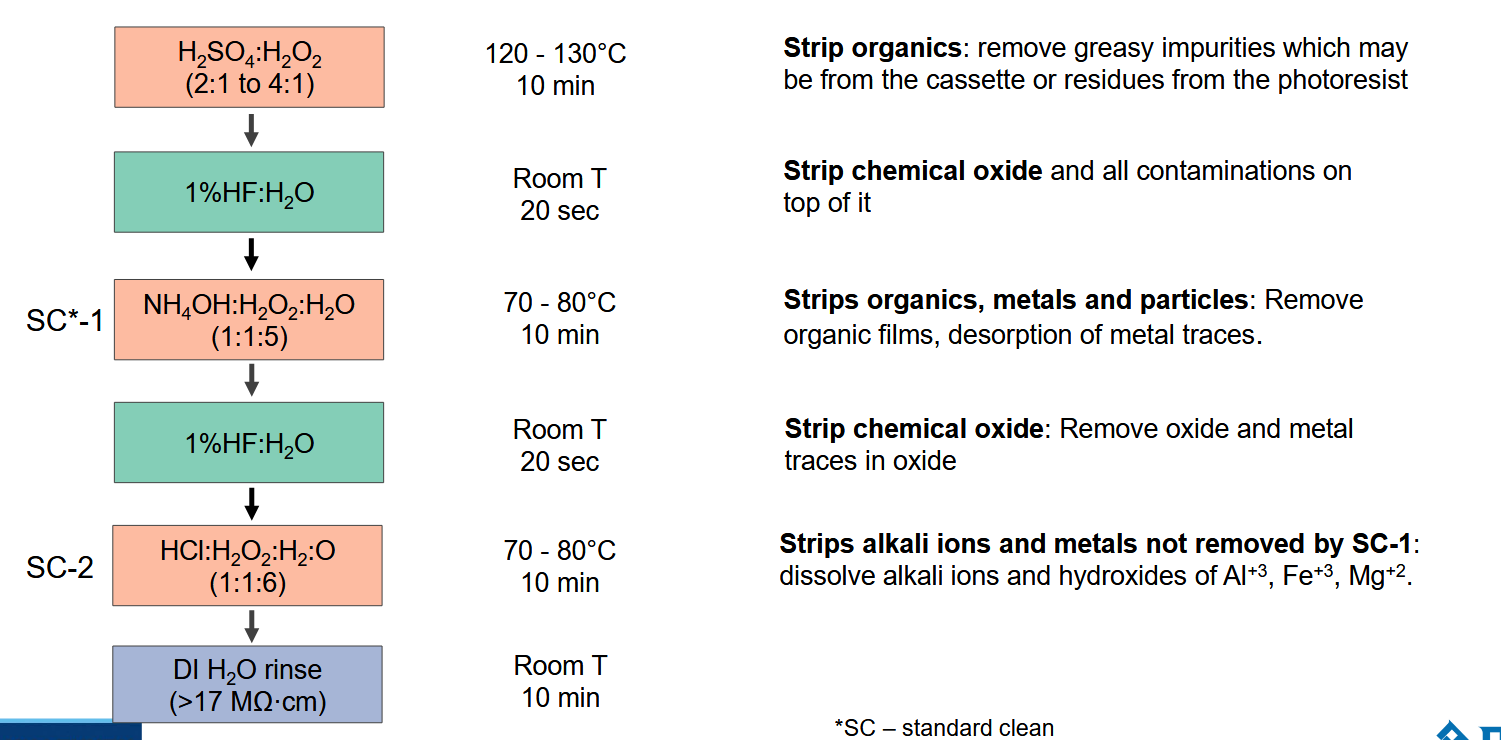
\includegraphics[keepaspectratio]{image-6.png}}\{.width=50\%\}

After this we can apply some HMDS to remove the OH group at the top of
the wafer to make the photoresist sticks better. We must also apply some
anti-reflective coating to avoid the UV light to strike unwanted area.

\subsubsection{Resist spinning}\label{resist-spinning}

We drop a little bit of the photoresist and then spin it faster to make
it a nice and even coat:

\[
T = \frac{K C^\beta \eta^\gamma}{\omega^\alpha}
\]

The thickness is \(0.05-100 \mu m\). The thickness varies due to step on
the wafer (previously deposited material).

\pandocbounded{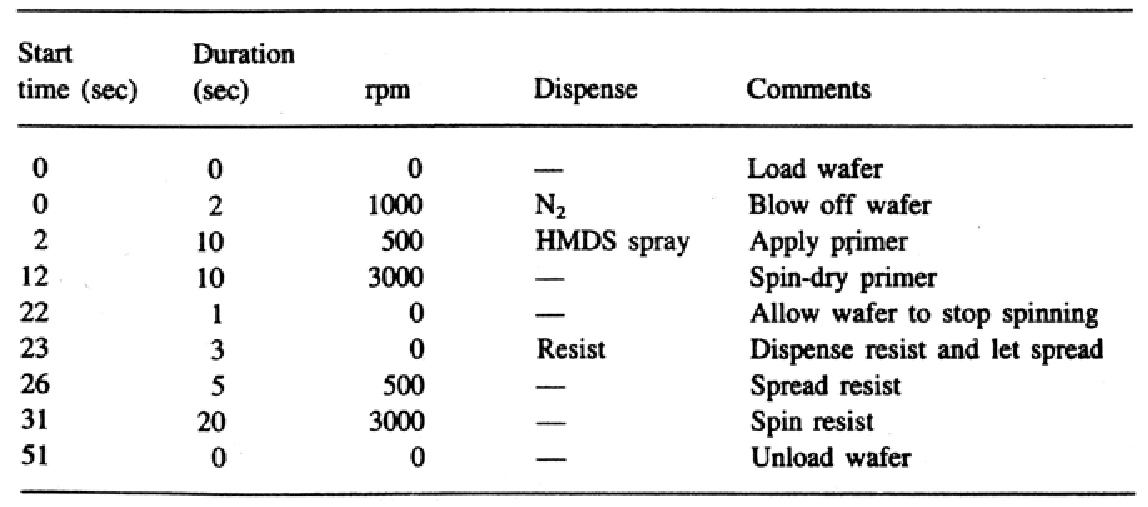
\includegraphics[keepaspectratio]{image-7.png}}\{.width=50\%\}

We can also use some \emph{spray coating} to spray and rinse through a
nozzle. The step coverage is better and more uniform. There is also dip
coating and laminating while they are less used in this industry.

After this we usually do some soft baking to improve resolution. If too
long we may decompose the resist watch out !

\begin{itemize}
\tightlist
\item
  few mins at 100C
\item
  30 mins in a convection oven
\end{itemize}

\subsubsection{Optic}\label{optic}

PSM is a prime example to improve resolution. With ARC we also trap some
lights in the resist creative some over exposed and ripple in the
sidewalls.

So we usually bake PEB to improve the sidewalls ripple ! We use some OPC
to correct and get the desired shape that may looks different on the
mask. Usually we print on a metal on chrome mask using an e-beam. Either
we use a master mask and directly use it to print on the wafer or we
first use the master mask to create a larger mask with multiple master
mask print on it. Reduction by \textbf{4 to 5} times reduction from mask
to wafer !!!

3 types of printing

\begin{enumerate}
\def\labelenumi{\arabic{enumi}.}
\tightlist
\item
  Contact printing: Mask is touching the wafer

  \begin{itemize}
  \tightlist
  \item
    Better resolution (less diffraction)
  \item
    Mask wear and wafer damage
  \end{itemize}
\item
  Proximity printing: not touching this time

  \begin{itemize}
  \tightlist
  \item
    Lower resolution
  \item
    Better mask lifetime
  \end{itemize}
\item
  Project printing: uses a set of lenses to focus on the mask and then
  on the wafer

  \begin{itemize}
  \tightlist
  \item
    Expensive technique but best of both
  \end{itemize}
\end{enumerate}

\subsubsection{Mask and formulas}\label{mask-and-formulas}

The most important metrics are:

\begin{itemize}
\tightlist
\item
  \textbf{Critical Dimension}: \(CD = k1 \frac{\lambda}{NA}\)
\item
  \textbf{Numerical Aperture}: \(NA = n sin(\theta)\)
\item
  \textbf{Depth of Focus}: \(DOF = k_2 \lambda/NA^2\) where \(k_2 < 1\)
\end{itemize}

\pandocbounded{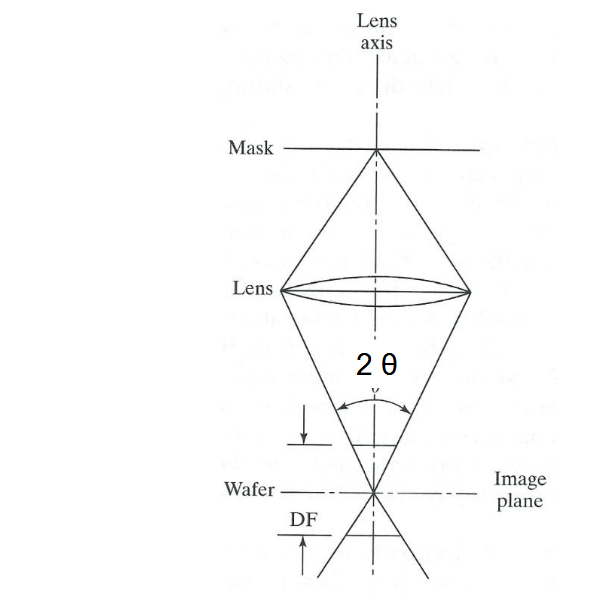
\includegraphics[keepaspectratio]{image-8.png}}\{.width=50\%\}

So clearly, we can see why having a small wavelength matters to get
better precision. To improve again we can use a wider \(\theta\).

With the DOF, some part could be in focus while other not which is
really problematic. We can't have a nice and uniform resolution accross
multiple lengths.

\subsubsection{Lights}\label{lights}

\pandocbounded{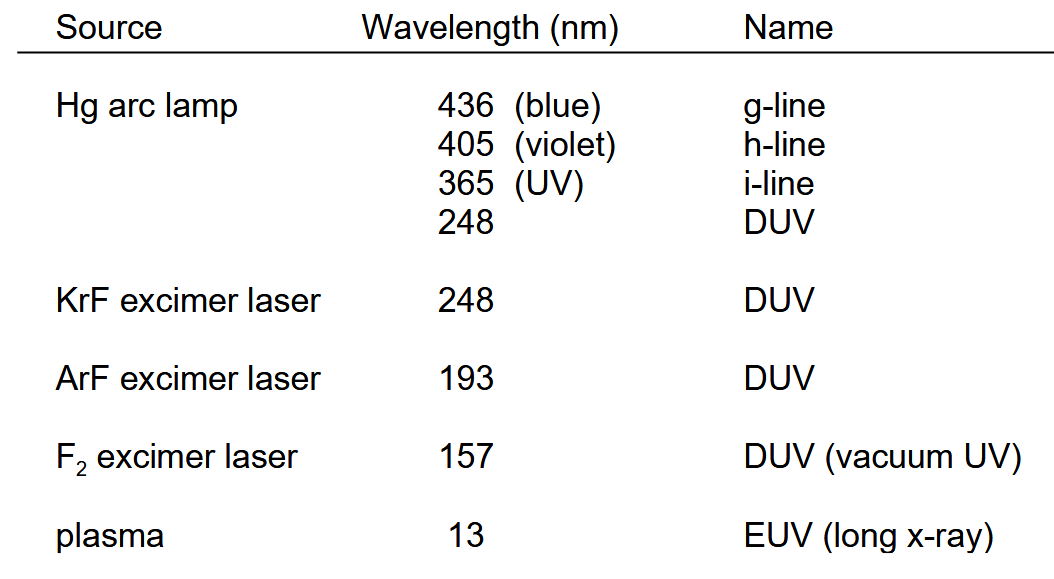
\includegraphics[keepaspectratio]{image-9.png}}\{.width=50\%\}

\subsubsection{Double patterning}\label{double-patterning}

We can use two mask to get virtually smaller features by combining those
two together.

\begin{itemize}
\tightlist
\item
  LELE: reduces \(k1\), double the cost since double patterning. Overlay
  issue :((
\item
  SADP: self aligning. Simply use dummy fill then add THICKKK sidewalls,
  etch it a lil, remove dummy and boom 2 pattern for the price of 1.
\item
  LFLE: based on a freezing process.
\item
  SAQP: close to SADP but pitches less than \(38 nm\)
\end{itemize}

\subsubsection{EUV}\label{euv}

We can't use lenses anymore. \textbf{7 mirrors with 70\% reflection per
mirror!} No pellicles that are EUV transparent yet.

To tune the linewidth we can change the exposure and development time.

For etching:

\begin{itemize}
\tightlist
\item
  wet etching: using acetone, IPA, water rinse. 2\% NaOH for positive
  resists
\item
  plasma etching: O2 plasma
\end{itemize}

\subsection{4 Oxidation, wet, dry}\label{oxidation-wet-dry}

SiO2 is forming a \emph{tetrahedral arrangement}. Can create some
amorphous structure too. The quality is determined based on the ratio of
bridging to non-bridging elements.

In elec, we use some amorphous.

\begin{longtable}[]{@{}cc@{}}
\toprule\noalign{}
Spec & Value \\
\midrule\noalign{}
\endhead
\bottomrule\noalign{}
\endlastfoot
density & \(2-2.3 gm/cm^3\) \\
\(\varepsilon_r\) & 3.9 \\
reflection index n & 1.5 \\
Breakdown field & \(10^7 V/cm\) \\
Trap/defect density at interface & \(10^{11} cm^{-2}\) \\
\end{longtable}

\subsubsection{Thermal oxidation}\label{thermal-oxidation}

Natural growth of a oxide exposed to air and enhanced by temperature.
Useful for:

\begin{enumerate}
\def\labelenumi{\arabic{enumi})}
\tightlist
\item
  implant/diffusion mask
\item
  surface passivation
\item
  isolation between transistors
\item
  key component of MOS structures
\item
  dielectric for multilevel interconnect
\item
  cleaning
\end{enumerate}

This grows in both way but slightly more outwards (\textbf{54/46}). SiO2
is 2.2 times larger than Si. Dry thermal is slower but better than wet
oxidation. Dry has a higher breakdown voltage --\textgreater{}
\(5-10 MV/cm\) so really good for gate oxide (since they are getting
smaller and smaller)!

For \(.5\mu m\) @ 1200C :

\begin{itemize}
\tightlist
\item
  Dry: 6 hours
\item
  Wet: 1 hour
\end{itemize}

We can have some interface issue as the step is not exactly the same and
so the development won't be equal. Can use color to determine the
thickness:

\begin{longtable}[]{@{}cc@{}}
\toprule\noalign{}
Thickness (\(\mu m\)) & Color \\
\midrule\noalign{}
\endhead
\bottomrule\noalign{}
\endlastfoot
0.07 & Brown \\
0.31 & Blue \\
0.39 & Yellow \\
0.41 & Light orange \\
0.47 & Violet \\
\end{longtable}

\subsubsection{LOCOS}\label{locos}

To have some isolation between transistor. Reduces topography by 56\%.
use some Nitrite which has a higher thermal expansion than Si. Add
padoxide as stress release.

\begin{itemize}
\tightlist
\item
  Si3N4: \(100-200 nm\)
\item
  SiO2: padoxide: \(20-30 nm\)
\end{itemize}

Wet oxi creating bird beak and then removing those oxide.

\subsubsection{STI}\label{sti}

Use CVD for the oxidation and CMP of the oxide avoids bird's beak and
mechanical stress.

\pandocbounded{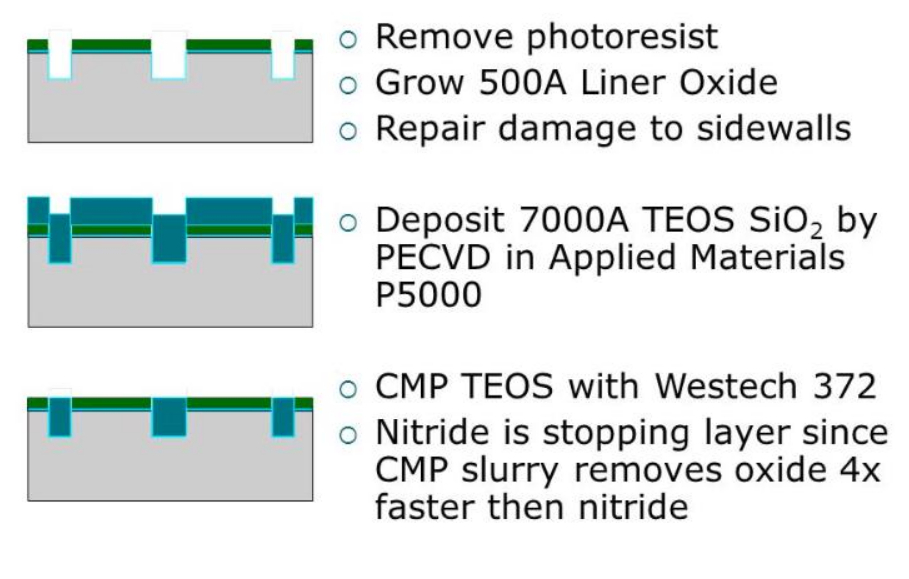
\includegraphics[keepaspectratio]{image-10.png}}\{.width=50\%\}

Better precision, the width drawn is the actual width. We also use some
dry oxidation which makes it better for large drive current.

\subsubsection{Doping}\label{doping}

We use either:

\begin{itemize}
\tightlist
\item
  gas, coating or ion implementation \#\#\#\# Diffusion Theory
\end{itemize}

We have a diffusion \emph{flux} of \emph{impurities} in one dimension.
(We are always using x as the vertical direction of diffusion).

\[\begin{aligned}
    F &= - D \frac{\partial C(x,t)}{\partial x} & D &= D_0 exp\left( \frac{-E_{\alpha}}{kT} \right)
\end{aligned}\]

We have \(D\) that is the \emph{diffusion coefficient} in \(cm^2/s\).
\(C\) is the dopant concentration per unit volume. We have \(D_0\) that
is the diffusion coefficient in \(cm^2/s\) at infinite temperature and
\(E_\alpha\) is the activation energy in \(eV\).

At low concentrations of dopant in silicon (\(10^{12} - 10^{16} cm^3\))
can be seen as constant. With this simplification, we can easily solve
the equation, we also see that gold, coper, ... have high diffusion
coefficient which is why we tend to avoid such metal in the clean room.

If we do not have a source or sink of the impurity, we know that the
\emph{change in impurity concentration with time must equal the local
decrease of diffusion flux}:

\[\begin{aligned}
    \frac{\partial C}{\partial t} &= - \frac{\partial F}{\partial x} = \frac{\partial}{\partial x} \left( D\frac{\partial C(x,t)}{\partial x} \right) & \frac{\partial C}{\partial t} &=  D\frac{\partial^2 C(x,t)}{\partial x^2} \text{ if D cst}
\end{aligned}\]

There are 2 methods of diffusion:

\begin{enumerate}
\def\labelenumi{\arabic{enumi}.}
\item
  \ul{Constant-surface-concentration:} using vapor, we have a constant
  concentration of dopants at the surface.
\item
  \ul{Constant-total-dopant:} thin layer, we have constant amount of
  impurity at the surface.
\end{enumerate}

\paragraph{Constant-surface-concentration}\label{constant-surface-concentration}

\[\begin{aligned}
    \text{Init: } C(x,0) &= 0 & C(0,t) &= Cs & C(\infty, t) &=0\\
    C(x,t) &= C_S erfc\left( \frac{x}{2\sqrt{Dt}} \right) & erfc(z) &= 1-erf(z) & erf(z)&=\frac{2}{\sqrt{\pi}}\int_0^\pi e^{-y^2} dy
\end{aligned}\]

We have \(\sqrt{Dt}\) that is called the \emph{diffusion length} in
\(cm\). The total number of dopant atoms per unit area that has diffused
into the semiconductor is given by:

\[Q(t) = \int_{0}^\infty C(x,t) dx = \frac{2}{\sqrt{\pi}} C_s \sqrt{Dt} \approx 1.13 C_s \sqrt{Dt}\]

\paragraph{Constant-total-dopant}\label{constant-total-dopant}

\[\begin{aligned}
    C(x,0) &= 0 & \int_0^\infty C(x,t) dx &= \phi & C(\infty, t) &= 0\\
     & & C(x,t) &= \frac{\phi}{\sqrt{\pi D t}} exp \left( - \frac{x^2}{4 D t} \right)
\end{aligned}\]

Where \(\phi\) is the \emph{total amount of dopant} per unit area. So
the surface concentration (\(x=0\)) is \(\phi / \sqrt{\pi Dt}\).

We usually use those two methods and we call this a \emph{two step
diffusion process}. a pre-deposition diffused layer is first formed
using constant-surface-concentration condition. Then a drive-in (or
redistribution) diffusion is used using constant-total-dopant condition.

For most practical cases the diffusion length for the pre-deposition
stage is much smaller than the diffusion length of the drive-in
diffusion. This allows to make deep junctions, e.g.~for wells for CMOS.

\pandocbounded{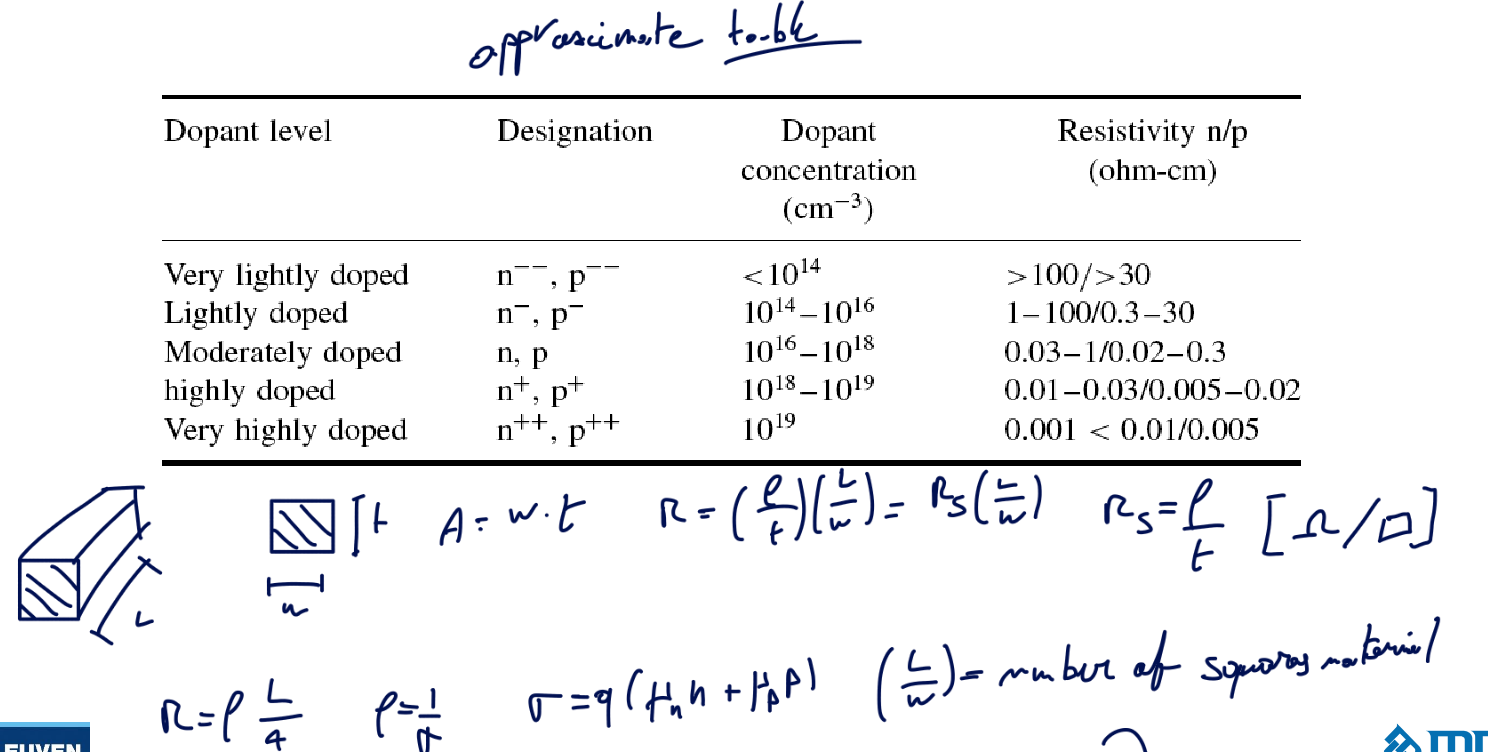
\includegraphics[keepaspectratio]{image-11.png}}\{.width=50\%\}

We also need a minimum mask width to be able to absorb all those ions in
the doping process.

\pandocbounded{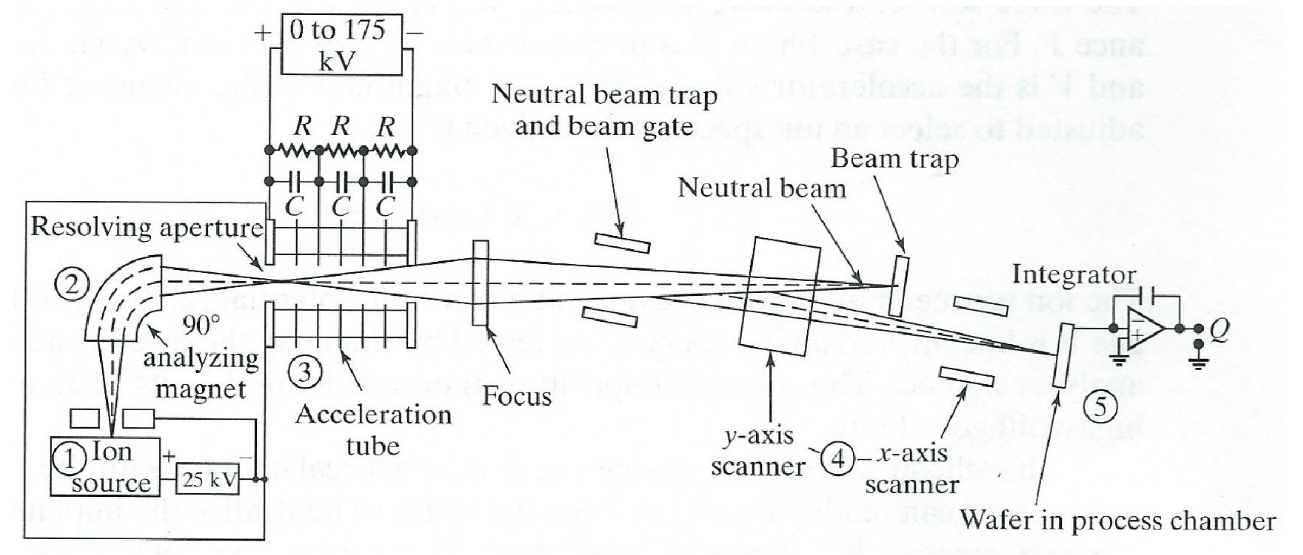
\includegraphics[keepaspectratio]{image-12.png}}\{.width=50\%\}

\subsubsection{Ion Implantation}\label{ion-implantation}

The source is at around \(25 kV\) and the high voltage accelerator goes
above \(> 5MeV\). There will be some undercut as the path traveled
inside won't be straight and it will bounce. So th depth is a gaussian.
Can have special behavior where the ion travels all the way through the
lattice without bouncing.

\[N(x) = N_p exp \left( - \frac{(x-R_p)^2}{2 \Delta R_p^2} \right) \qquad N_p = \frac{\phi}{\sqrt{2 \pi} \Delta R_p}\]

\(\Delta R_p\) being the \emph{projected straggle} distance from the
peak with concentration reduced by \(40\%\).

Need some \textbf{rapid annealing} to repear the lattice after, will
spread out the concentration sadly.

\subsection{5 Etching, wet, dry, plasma,
DRIE}\label{etching-wet-dry-plasma-drie}

Wet etching is cheaper \textbf{10k} while dry etching is \textbf{1M}.
But wet etching is mostly isotropic meaning it goes into all direction
which leads to al ot of undercut.

Wet etching is quite simple using a bath and a quick dump to stop
precisely the etching and using some nozzle to stop any reaction. This
limits the feature size as too close gaps can be bridged during the
process \(< 3 \mu m\). We use \textbf{HF} for SiO2 \textbf{WATCH OUT} it
will get through your skin without any pain but starts attacking your
bones after.

\subsubsection{Anisotropic}\label{anisotropic}

It has a prefered lattice orientation that will be etched faster. Dry
etching is a combination of temperature and vacuum.

\pandocbounded{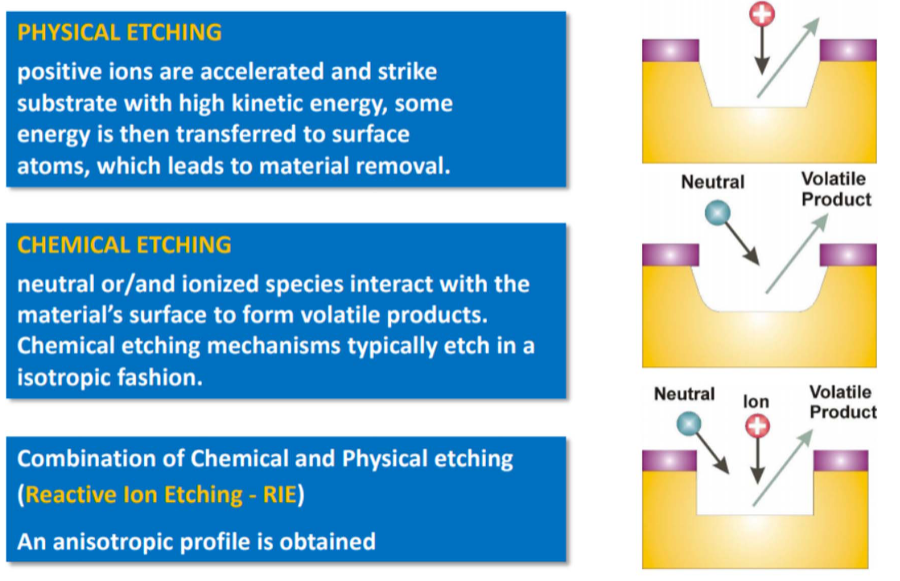
\includegraphics[keepaspectratio]{image-13.png}}\{.width=50\%\}

\paragraph{Plasma Etching}\label{plasma-etching}

Same amount of positive and negative charges but a different number of
unionized molecules. Large electric field applied to a gas up to the
\textbf{breakdown of the gas}.

\pandocbounded{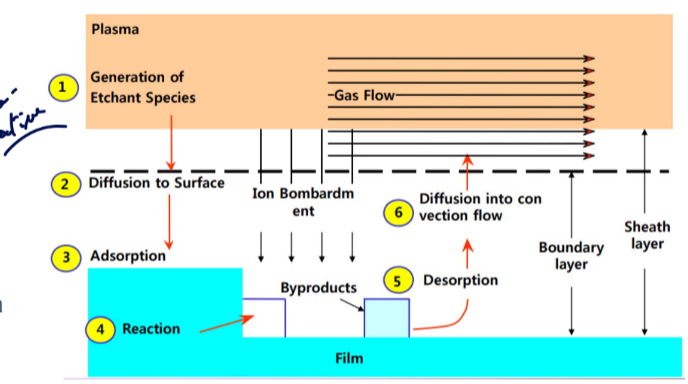
\includegraphics[keepaspectratio]{image-14.png}}\{.width=50\%\}

Needs \textbf{high kinetic energy and chemical reactions}. There are
about \(10^{15} cm^{-3}\) neutral species and
\(10^8 - 10^{12} cm^{-3}\). Ions go on the surface and strike it to
remove some molecules.

\pandocbounded{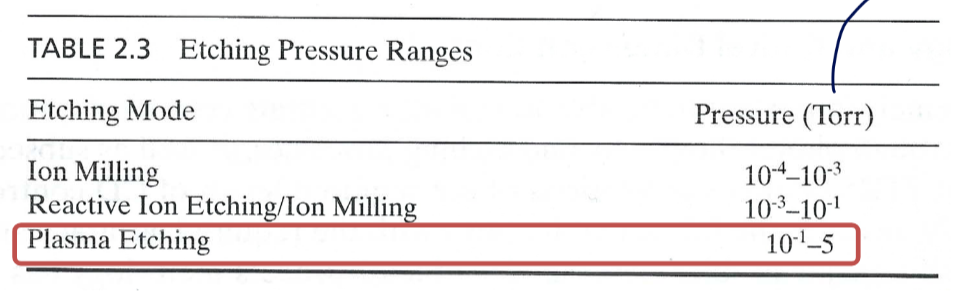
\includegraphics[keepaspectratio]{image-15.png}}\{.width=50\%\}

RIE will create a DC bias to accelerate the ions and add some extra
kinetic energy towards the substrate. This is a combination of
\textbf{chemical and sputter etching}. The chemical is purely isotropic
and with little electrical damage while the sputtering is anisotropic
and slower (this is ion milling).

\pandocbounded{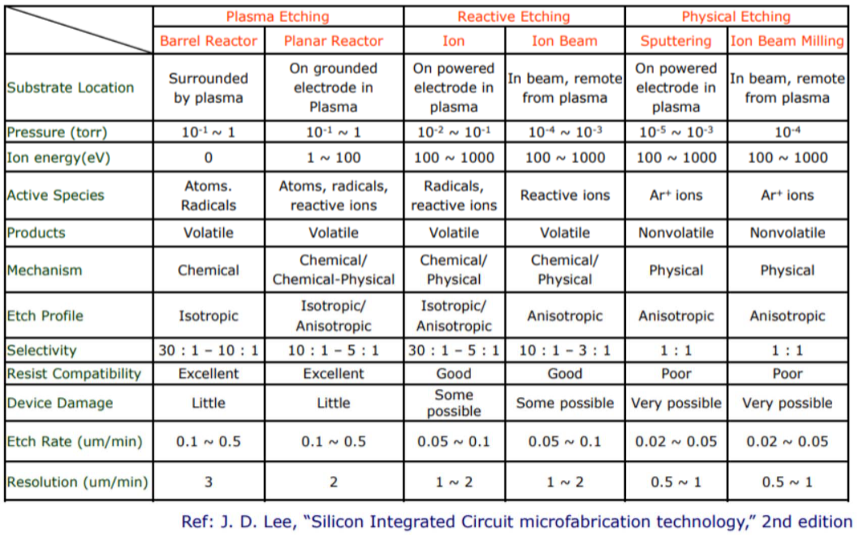
\includegraphics[keepaspectratio]{image-16.png}}\{.width=50\%\}

RIE is a sophisticated and complex process where changing a single
parameters could impact the total chain of the reaction leading to
issues.

\paragraph{DRIE}\label{drie}

With this method we can obtain an \textbf{aspect ratio of 20-50} and the
etch rate is around \(> 10 \mu m/min\).

\subsection{6 Interconnect}\label{interconnect}

Aluminium has a fairly low melting point at around \(577 C\). The
interconnect and contact Al is done during the same step. But Al has the
tendency to fall into the crevices left by the Si that diffuses inside
th Al. So add 1\% of Si in Al or use barrier material like TiW.

We want to further reduce the contact resistance so we must employ some
alloy mixed with Si. We are using the fact that Si diffuses into the
metal so then we can remove the non-reacted metal and boom we got some
nice salicide.

\subsubsection{Electromigration}\label{electromigration}

If the track is not made thick enough, the electrons can take with them
some bits of the material and move them further. Creating gaps and
increasing the resistance. One solution is to add 4\% copper to the mix
making the interconnect Al-Cu-Si, 95-4-1.

\subsubsection{Interconnect}\label{interconnect-1}

For stack up layer we may be misaligned so we must make the via wider
each time as we go up or add some offset.

After making an interconnect we tend to planarize to have a fresh and
flat surface to work on. So we will use some CMP process to make
everything smooth. Damascene process is based on this idea.

We may need to add some dummy fill oxide to ensure a global planarity
after the CMP. Or another technique is using some \emph{reverse tone
litho} and already pre-etch oxides that are on top of other stuff and
are too wide.

But at some point, Al is not fast enough, too much delay for a small
feature size. We had to go for Copper even though it has a high
diffusivity. Issue with adhesion, \ldots{}

So we have to add a \textbf{seed layer} to avoid this diffusion. This
seed layer is a thin conductive layer and then we can put the big chunk
of copper.

\pandocbounded{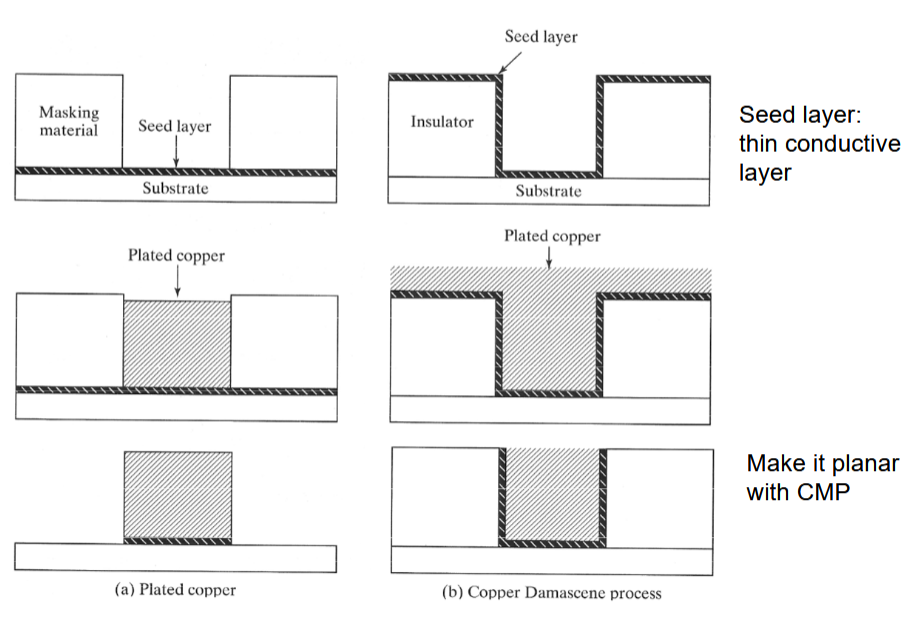
\includegraphics[keepaspectratio]{image-17.png}}\{.width=50\%\}

Dual damascene is used when creating those wider form of via. Good for
vias and interconnect traces.

It is often hard to etch metal so we can use lift off where we first
apply the photoresist and then the metal. Finally we simply need to etch
the mask and everything should come off. Here we want a \textbf{bad step
coverage}.

\subsection{7 Ic Processing Overview}\label{ic-processing-overview}

\emph{up to slide 47}

The biggest issue currently is the non-aligning gate. With the Aluminium
gate we \textbf{can't use some ion implantation} since it is happening
above the melting point of the gate. So the process is trickier and same
for etching, only low temp process --\textgreater{} mostly isotropic and
wet. Good for \(>5 \mu m\).

We ditched it to go for some nice polygate, can use fancier process and
they are self aligning. Good for \(< 10 \mu m\).

\subsubsection{Al vs poly}\label{al-vs-poly}

Here, we first need to dope the substrate before depositing the gate as
we usually go into melting point order. From high to low.

For poly, we first deposit the gate and then dope the wafer. This will
make sure that drain and source are already aligned !

Here, we still do some LOCOS operation to isolate our PMOS and NMOS. And
then once the base is laid down we can start adding our poly-gate. We
apply all the tips and informations we have seen in the course to build
a good transistor.

\pandocbounded{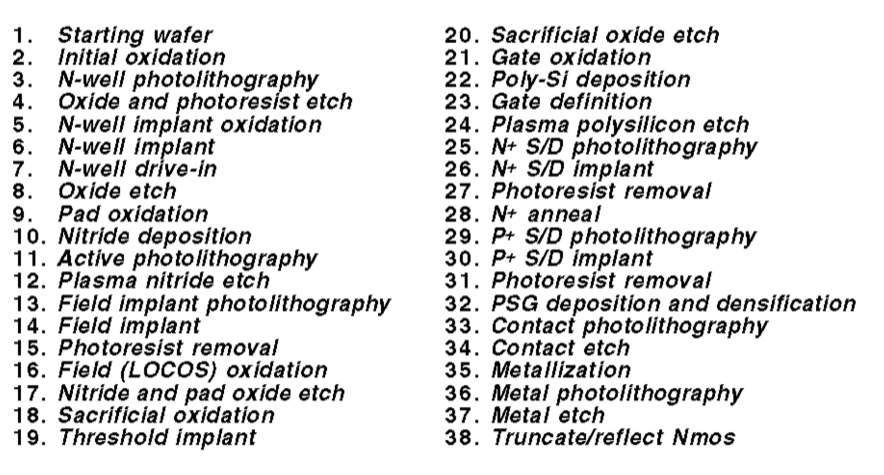
\includegraphics[keepaspectratio]{image-18.png}}\{.width=50\%\}

\subsubsection{Latch-up issue}\label{latch-up-issue}

For this, it is important to use some good EPI and STI to avoid any
cross connection resulting in a possible \emph{thyristor}.

\pandocbounded{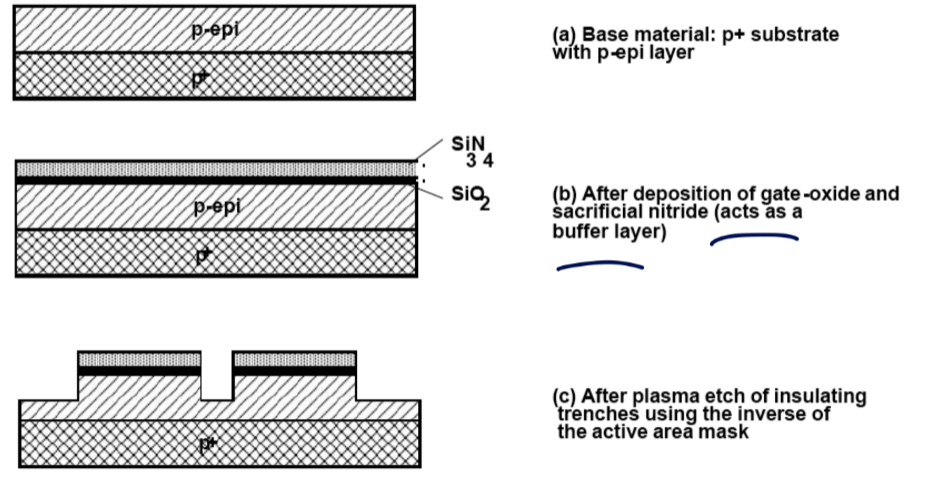
\includegraphics[keepaspectratio]{image-19.png}}\{.width=24\%\}

\pandocbounded{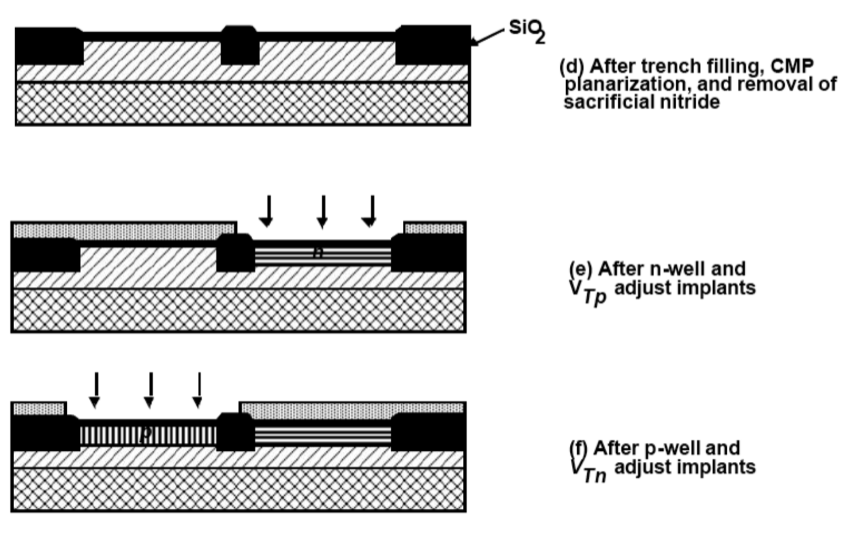
\includegraphics[keepaspectratio]{image-20.png}}\{.width=24\%\}

\pandocbounded{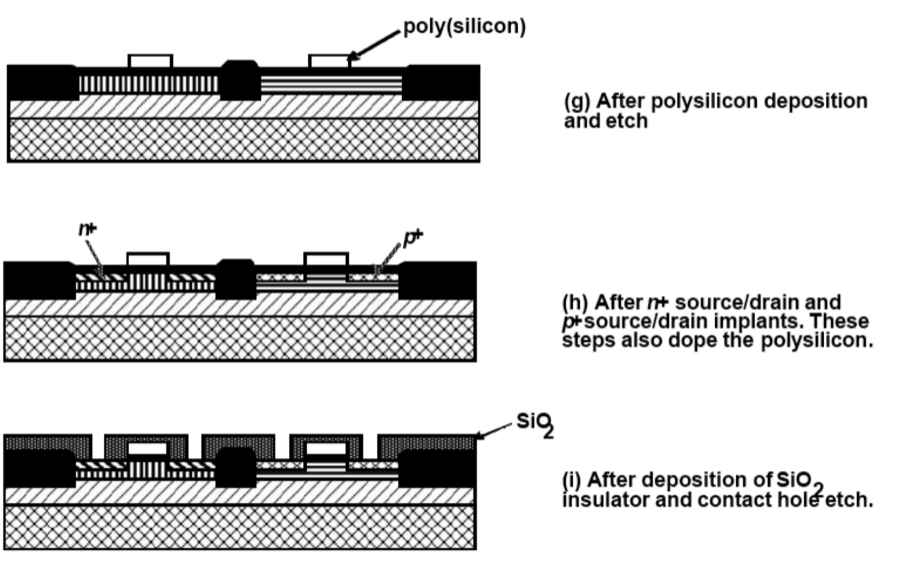
\includegraphics[keepaspectratio]{image-21.png}}\{.width=24\%\}

\pandocbounded{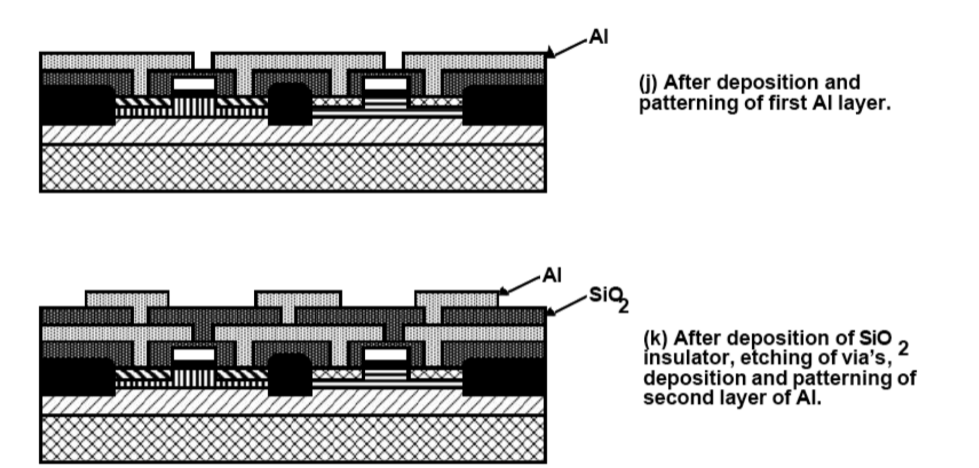
\includegraphics[keepaspectratio]{image-22.png}}\{.width=24\%\}

\subsubsection{Hot carrier effect}\label{hot-carrier-effect}

TODO

\subsubsection{Contacting issues}\label{contacting-issues}

For this we again use some salacides, by blanket depositing, a bit of
the metal will react and simply diffuse. The other non-reacted can be
targeted and removed. Contact is now made easy. We usually do some
\textbf{annealing} to improve the resistivity of the contact.

\paragraph{Gate last}\label{gate-last}

Here we first add a dummy gate and at the end att eh contact of the gate
using some metal, replacement of poly-silicon.

\subsection{8 Packaging}\label{packaging}

Not seen this year.

\end{document}
